%%%%%%%%%%%%%%%%%%%%%%%%%%%%%%%%%%%%%%%%%%%
\section{Installing The Environment}
The environment we use in this book is developed on top of the \sq environment. \sq is a rich open-source and multimedia system entirely written in Smalltalk. 
\sq runs exactly the same on all the platforms, however to simplify your start we prepared some platform dependent zipped files. Note that the principle is exactly the same on Mac, PC, or any other platform only the decompressing tools and the way to invoke \sq may differ. Basically you decompress the file, drag the file named \ct{ReadyToUse.image} on the \ct{Squeak application}, and this is it. You should then get the system as shown in Figure~\ref{fig:firstEnvironment}. Now let us look at each of the steps one by one. Note that you may get files with slightly different names but it should work. 

\paragraph{On Mac.}
You should have a file named \ct{readyToUseForMac.sit}, an archive or \ct{readyToUseForMac.sea} a self-extracting archive. This file contains the complete environment used in this book. When you decompressed this file (by double-clicking on it), you should obtain 4 files on Mac OsX as shown by Figure~\ref{fig:macfiles}. You should identify two files: the file named \ct{ReadyToUse.image} and the \emph{Squeak application} file (the one without extension in Figure~\ref{fig:macfiles} it is named \ct{Squeak 3.2.8Beta9}).

\begin{figure}[!h]\centerline{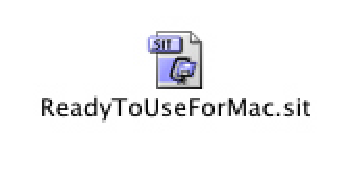
\includegraphics{readyToUseForMacZip}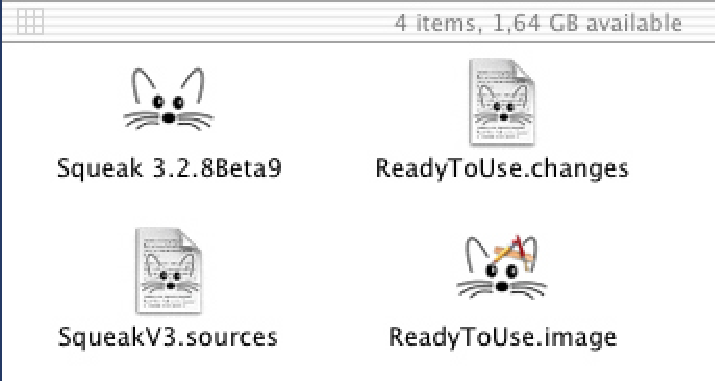
\includegraphics[width=9cm]{macFiles}}
\caption{The files for the ready to use environment. Left: the zipped files. Right: the unzipped files.\label{fig:macfiles}}\end{figure}

\paragraph{On Windows.}
You should have a file named \ct{readyToUseForMac.zip}, an archive. This file contains the complete environment used in this book. When you decompressed this file using Winzip, you should obtain 4 files as shown by Figure~\ref{fig:pcfiles}. You should identify two files: the file named \ct{ReadyToUse.image} and the \emph{Squeak application} file (the one without extension in Figure~\ref{fig:macfiles} it is named \ct{Squeak 3.2.8Beta9}.


\begin{figure}[!h]\centerline{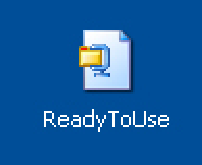
\includegraphics{zipPC}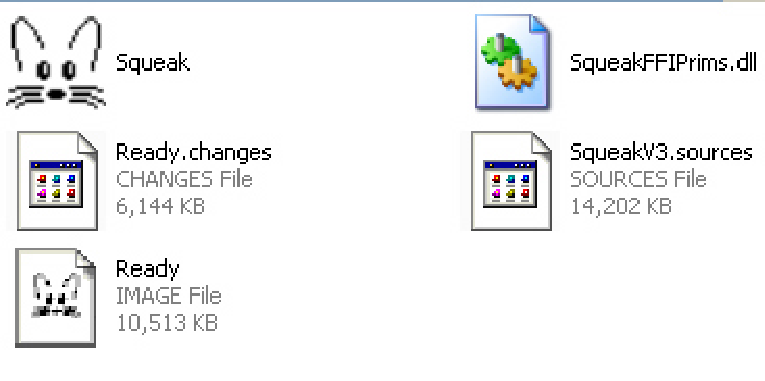
\includegraphics[width=9cm]{readyPC}} 
\caption{The files for the ready to use environment on PC. Left: the zipped files. Right: the unzipped files.\label{fig:pcfiles}}
\end{figure}


\section{Opening the Environment} 
To open the environment, drag the file \ct{ReadyToUse.image} on the \emph{Squeak application} as shown by Figure~\ref{fig:dropImage}. You should get the environment shown in Figure~\ref{fig:firstEnvironment}.

\begin{figure}[!h]\centerline{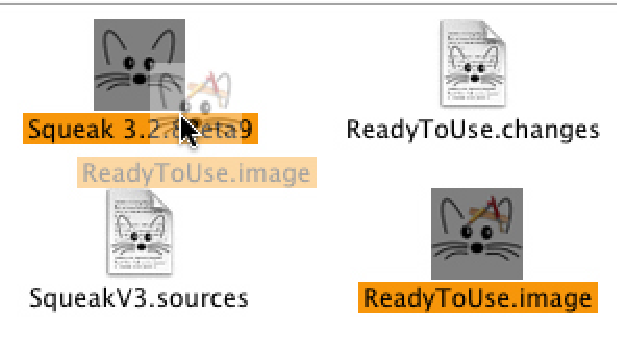
\includegraphics[width=8cm]{dropImage}  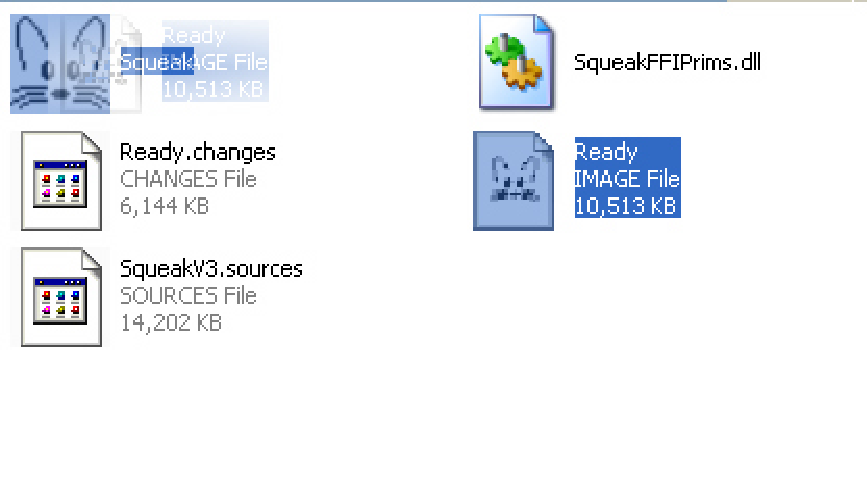
\includegraphics[width=8cm]{readyDD}} 
\caption{Dragging and dropping the \textit{image} file on the 
\textit{Squeak application} to open on Mac (left) on PC (right).\label{fig:dropImage}}
\end{figure}


The environment can be opened by simply double-clicking on the \textit{image} file. However, such a practice has several disavantages: you should identify the \emph{Squeak application} and something another application may by accident try to use the image. Moreover it can lead you to trouble when you have multiple installations of different versions of \sq. So we suggest to always open the environment by dragging and dropping the image file on the \emph{Squeak application} file or alias to it. Note that if you have space problem you can use an alias to the SqueakV3.sources file as this file can be shared between multiple installations. 



\begin{largecadre}{To start the environment. 
Drag and drop the file terminating with the .image extension into the squeak application.}
\end{largecadre}
 